% Suggested revision of Section 4.1 (qLMPC Design and Application), lines 46-543 of
% 04_WindTurbineControl_02_notBold.tex, aligned with the qLMPC code (10 augmented states,
% per-sample rate limits, plant actuator time constants). Drop-in replacement for those lines.
\section{qLMPC Design and Application}\label{sec:quasiLPVMPCDesign}
Wind turbine controller design in above rated region focuses on smooth power control and in the below rated region on power optimization, as described in \cite{Bianchi2007}. Generator speed reference tracking is achieved using two control inputs: the collective blade pitch angle $\beta_{0,\text{ref}}$ and the generator torque reference $T_{g,\text{ref}}$. The baseline controller consists of two SISO controllers, one for generator torque and one for blade pitch control, see Section~\ref{sec:WindTurbineControl}. These can be replaced by a MIMO qLMPC power controller, see Figure \ref{fig:BlockMPC}. The qLMPC is designed to track rotor and generator speed references while minimizing changes in the control inputs, resulting in smoother power output and reduced tower movement compared to the baseline. DEL reduction is not an explicit objective of the qLMPC design. However, the five evaluation criteria used to compare all control strategies introduced in Section~\ref{subsection Control Objectives}, i.e., blade and tower DEL, power mean and variance, and actuator activity, are also calculated for this controller to enable a direct comparison with the IPC and AALC designs.

\begin{figure}[ht]
    \centering
    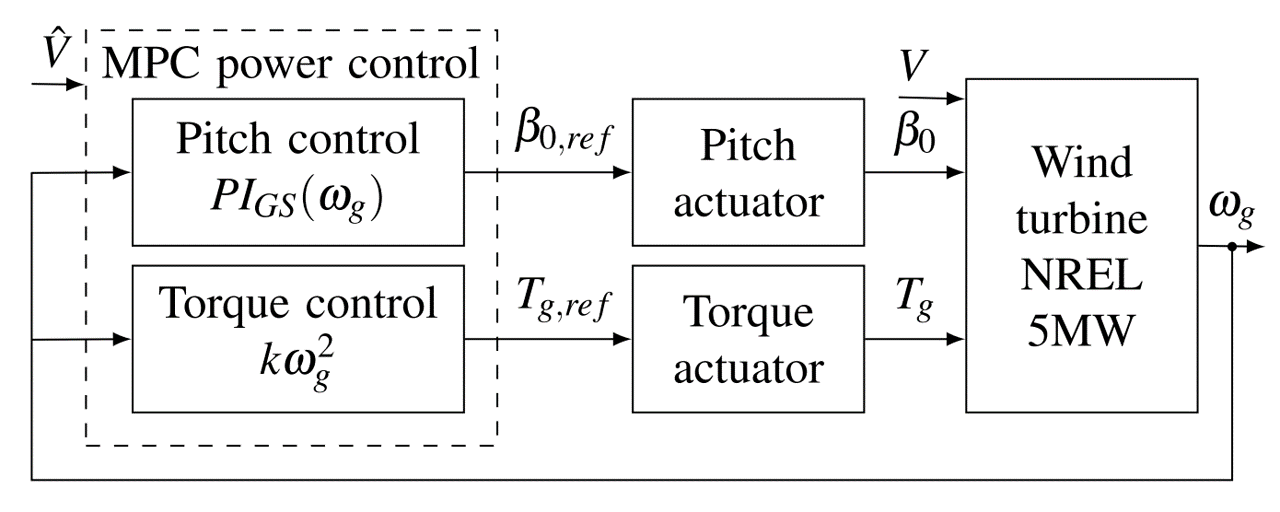
\includegraphics[width=0.8\textwidth,trim={0 0cm 0cm 0.3cm},clip]{figures/Figures_ADi/turbineMPC.png}
    \caption[Block diagram of the closed-loop wind turbine control structure with qLMPC replacing the baseline PI controller]{Block diagram of the closed-loop wind turbine control structure with qLMPC (dashed box) replacing the baseline PI controller (solid line)}
    \label{fig:BlockMPC}
\end{figure}

In this work, the velocity based approach from \cite{cisneros2020velocity}, presented in section \ref{windTurbineModel} of this thesis, is applied: A $3^{rd}$ order wind turbine model, used as the basis for quasiLPV based MIMO controller design in \cite{Bianchi2007}, is implemented with some minor changes. To model the main dynamics, it is sufficient to consider the slip angle $\theta_s$, the rotor and generator speed $\omega_r$ and $\omega_g$. The same states are considered here, but three modifications were made:
\begin{enumerate}
    \item A filtered generator torque $T_g^{\prime} = T_{g,\text{ref}}$ is introduced as an additional state to eliminate direct throughput, i.e., to avoid a non-zero feedthrough matrix \( \bm{D} \). This fourth state enables the use of the optimization framework for reference tracking and disturbance rejection proposed in \cite{cisneros2020velocity}. Incorporating a filtered control input as an additional state is a common practice, and is, for example, also employed in the MPC algorithm implemented in WFSim \cite{boersma2018control}.    
    \item Reference generator torque $T_{g,\text{ref}}$ is used as a control output signal and plant input signal. In \cite{Bianchi2007}, the second control input is the zero torque speed $\omega_Z$ which is linearly dependent on the generator torque $T_{g}$. The reference torque is selected as it is the format of expected input signal to the wind turbine in the FAST implementation. The optimal trajectory of the reference generator torque  $T_{g,\text{ref}}$ over a prediction horizon is calculated based on an optimal reference signal $r_{\beta}$ which is itself calculated from the wind speed.
    \item A desired pitch signal $r_{\beta}$ is used as a reference for the prediction horizon in the MPC optimization to calculate the optimal controller output pitch signal $\beta_{0,\text{ref}}$. In \cite{Bianchi2007}, a reference value for the generator speed is tracked. This choice was made to directly optimize the two actuators to avoid handling the large difference in dynamic bandwidth of the actuators and the plant dynamics in the optimization calculation. Identical to the filtered generator torque, a filtered pitch $\beta_0^{\prime} = \beta_{0,\text{ref}}$ is introduced as a fifth state.
\end{enumerate}
%
The resulting states, input and output vectors are given below. As before, different indices are used for the generator speed in the high-speed shaft, denoted $\omega_g$, and the low-speed shaft, $\omega_{gr}$. In the state vector, the generator speed in the low-speed shaft is used as it operates in the same reference system as the rotor speed $\omega_r$:
\begin{align}\label{eq:xMPCyMPC}
    \bm{x}_{\text{MPC}} =[\theta_{s}  \quad {\omega}_r \quad {\omega}_{gr} \quad T_g^{\prime} \quad \beta_0^{\prime} ]^T  \in \mathbb{R}^{5 \times 1},   \quad \bm{y}_{\text{MPC}} = [T_{g,\text{ref}} \quad  {\beta}_{0,\text{ref}}]^T  \in \mathbb{R}^{2 \times 1}.
\end{align}
%
The nonlinear dynamics describing changes in the three turbine states are:
\begin{align}
    \dot{\theta_s}(t)&={\omega}_r(t)-{\omega}_{gr}(t) \label{eq:NLDyn1}\\
    \dot{\omega}_r(t)&=-\frac{K_{sr}}{J_r}\theta_s(t)-\frac{B_{sr}}{J_r}{\omega}_r(t)+\frac{B_{sr}}{J_r}{\omega}_{gr}(t)+\frac{T_r({\omega}_r, \beta, v)}{J_r}\\
    \dot{\omega}_{gr}(t)&=\frac{K_{sr}}{J_{gr}}\theta_s(t)+\frac{B_{sr}}{J_{gr}}{\omega}_r(t)-\frac{B_{sr}}{J_{gr}}{\omega}_{gr}(t)-\frac{N_gT_g(t)}{J_{gr}} \label{eq:NLDyn3} \\
 %   \dot{ T}^{\prime}_{g} &= -\frac{1}{ \kappa}T_{g} +\frac{1}{ \kappa}T_{g, ref}\\
%    \dot{\beta}^{\prime}_& = -\frac{1}{ \tau}\beta^{\prime} +\frac{1}{ \tau}\beta_{g, ref}
\end{align}
%
To avoid having to derive a grid of initial states for the different combinations of the state vector, a velocity based linearization is designed.
\subsection{Velocity-Based qLPV Model Linearization}
The velocity-based linearization method from \cite{cisneros2020velocity} is implemented for the model serving as the basis of the qLMPC design. The nonlinear system dynamics
\[
\dot{\bm{x}}_{\text{MPC}}(t) = \bm{f}_{\text{MPC}}(\bm{x}_{\text{MPC}}, \bm{w}_{\text{Mdl}}), \quad \bm{y}_{\text{MPC}}(t) = \bm{h}_{\text{MPC}}(\bm{x}_{\text{MPC}})
\]
are described by the relationship between the state and input derivatives: 
\begin{align*}
    \ddot{\bm{x}}_{\text{MPC}}(t) &= \nabla_{\bm{x}_{\text{MPC}}} \bm{f}_{\text{MPC}}(\bm{x}_{\text{MPC}}, \bm{w}_{\text{Mdl}}) \dot{\bm{x}}_{\text{MPC}}(t) + \nabla_{\bm{w}_{\text{Mdl}}}\bm{f}_{\text{MPC}}(\bm{x}_{\text{MPC}}, \bm{w}_{\text{Mdl}}) \dot{\bm{w}}_{\text{Mdl}}(t),\\
    \dot{\bm{y}}_{\text{MPC}}(t) &= \nabla_{\bm{x}_{\text{MPC}}}\bm{h}_{\text{MPC}}(\bm{x}_{\text{MPC}}) \dot{\bm{x}}_{\text{MPC}}(t).   
\end{align*}
By considering the derivatives instead of the original states, the need for storing steady-state vectors for input, output, and states at each operating point is omitted.
%

The continuous-time system, input, and output matrices,
\begin{align*}
      \bm{A}_c(\bm{\rho}_{\Rho}) &= \nabla_{\bm{x}_{\text{MPC}}} \bm{f}(\bm{x}_{\text{MPC}}, \bm{w}_{\text{Mdl}}),\\ 
      \bm{B}_c(\bm{\rho}_{\Rho}) &= \nabla_{\bm{w}_{\text{Mdl}}} \bm{f}(\bm{x}_{\text{MPC}}, \bm{w}_{\text{Mdl}}),\\ 
      \bm{C}_c(\bm{\rho}_{\Rho}) &= \nabla_{\bm{x}_{\text{MPC}}} \bm{h}(\bm{x}_{\text{MPC}}),
\end{align*}
where the scheduling parameter $\bm{\rho}_{\Rho}$ consists of the measurement values of  wind speed $V_{\infty}$, pitch angle $\beta_0$ and rotor speed $\omega_r$,
\[\rho_{P} = [V_{\infty} \quad {\beta_0} \quad {\omega}_{r} ]\in \mathbb{R}^{1 \times 3}, \]  
with the corresponding state vector $\bm{x}_{\text{MPC}}$ and output vector $\bm{y}_{\text{MPC}}$ as defined in Equation~\ref{eq:xMPCyMPC} and $w_{\text{Mdl}} = [V_{\infty} \; \; T_g  \; \; \beta_0]$. Although the control scheme is velocity-based, i.e., based on state derivatives or, in discrete time, state differences, the scheduling parameters are taken in their original non-derivative form. This is because the partial derivatives such as \( \partial T_r / \partial \omega_r \), \( \partial T_r / \partial \beta \), and \( \partial T_r / \partial V_{\infty} \), are functions of the current physical states, not their time derivatives.

The matrices depend on the physical parameters described in Section \ref{sec:MechanicalAerodynamicSubsystemModel} and can be set up from Equations~\eqref{eq:NLDyn1} to~\eqref{eq:NLDyn3}:  
\begin{equation}
    \begin{aligned}
        \bm{A}_c(\bm{\rho}_{\Rho}) &=
        \begin{bmatrix}
            0  & 1 & -1 & 0 & 0 \\ 
            -\frac{K_{sr}}{J_r}  & -\frac{B_{sr}}{J_r} + \frac{1}{J_r}\frac{\partial T_r}{\partial{\omega_r}} & \frac{B_{sr}}{J_r} & 0 & \frac{1}{J_r}\frac{\partial T_r}{\partial{\beta}} \\ 
            \frac{K_{sr}}{J_{gr}} & \frac{B_{sr}}{J_{gr}} & -\frac{B_{sr}}{J_{gr}} & -\frac{N_g}{J_{gr}} & 0 \\ 
            0 & 0 & 0 & -\frac{1}{\kappa} & 0 \\ 
            0 & 0 & 0 & 0 & -\frac{1}{\tau} 
        \end{bmatrix} \in \mathbb{R}^{5 \times 5},\\
\bm{B}_c(\bm{\rho}_{\Rho}) &=
\left[
\begin{array}{c|cc}
    0 & 0 & 0 \\
    \frac{1}{J_r}\frac{\partial T_r}{\partial V_{\infty}} & 0 & 0 \\
    0 & 0 & 0 \\
    0 & \frac{1}{\kappa} & 0 \\
    0 & 0 & \frac{1}{\tau}
\end{array}
\right]
=
\begin{bmatrix}
    \bm{B}_{c,V} & \bm{B}_{c,u}
\end{bmatrix}
\in \mathbb{R}^{5 \times 3}\\
        \bm{C}_c &=
        \begin{bmatrix}
            0 & 0 & 0 & 1 & 0 \\
            0 & 0 & 0 & 0 & 1
        \end{bmatrix} \in \mathbb{R}^{2 \times 5}.
    \end{aligned}
\end{equation}
%
The actuator time constants of the prediction model are set to the values of the first-order actuator models of the plant, see Equations~\eqref{eq:Tact} and~\eqref{eq:betaact}, i.e., $\tau = 0.05$\,s for the pitch and $\kappa = 0.01$\,s for the generator torque.
The wind affects the system through the first column of the input matrix, denoted here as $\bm{B}_{c,V}$. The wind speed $V_{\infty}$ cannot be controlled and only its current value is assumed to be known and constant over the prediction horizon. Nevertheless, the column $\bm{B}_{c,V}$ must be retained, as the change in wind speed $\Delta V_{\infty}$ is treated as a disturbance input between time steps. To reflect this structure, the input matrix $\bm{B}_c$ is partitioned into the wind disturbance input $\bm{B}_{c,V}$ in the first column and the control input influence $\bm{B}_{c,u}$ in the second and third columns. For implementation in the predictive controller, the wind-dependent column is moved into the system matrix as an additional state, since it represents a known but uncontrollable input.

This continuous LPV model needs to be discretized for its application in a real-time qLMPC design. The model in discretized form is:
\begin{align}\label{eq4:DiscreteForm}
    \Delta \bm{x}_{\text{MPC},k}(k+1) = \bm{A}_{k}(\bm{\rho}_\Rho)\Delta \bm{x}_{\text{MPC},k}(k) + \bm{B}_{k}(\bm{\rho}_\Rho) \Delta \bm{w}_{\text{Mdl},k}(k)
\end{align}
with the discretized system and input matrices $\bm{A}_k \in \mathbb{R}^{5 \times 5}$ and $\bm{B}_k  \in \mathbb{R}^{5 \times 3}$ dependent on scheduling parameter vector $\bm{\rho}_{P}$ at the $k^{\text{th}}$ sample.
%
%
As in \cite{cisneros2019wide} the 4$^{th}$ order discretized state space representation to derive the matrices  $\bm{A}_k$ and $\bm{B}_k$ is implemented as:
\begin{align*}
    \bm{A}_{k}(\bm{\rho}_\Rho) &= \frac{T_s^4}{24}\bm{A}_c^4(\bm{\rho}_\Rho) + \frac{T_s^3}{6}\bm{A}_c^3(\bm{\rho}_\Rho) + \frac{T_s^2}{2}\bm{A}_c^2(\bm{\rho}_\Rho) + T_s \bm{A}_c(\bm{\rho}_\Rho)+ I,\\
    \bm{B}_{k}(\bm{\rho}_\Rho) &= \frac{T_s^3}{24}\bm{A}_c^3(\bm{\rho}_\Rho)\bm{B}_c(\bm{\rho}_\Rho) + \frac{T_s^2}{6}\bm{A}_c^2(\bm{\rho}_\Rho) \bm{B}_c(\bm{\rho}_\Rho) + \frac{T_s}{2} \bm{A}_c(\bm{\rho}_\Rho) \bm{B}_c(\bm{\rho}_\Rho)
    + \bm{B}_c(\bm{\rho}_\Rho).
\end{align*}
%
The discrete-time outputs can be calculated as the sum of the former sampled outputs and their current change:
\begin{align*}
    T_g^{\prime} (k+1)= T^{\prime}_g(k)  + \Delta T^{\prime} _g(k+1), \quad \beta^{\prime}_0(k+1) = \beta^{\prime}_0(k) + \text{Act}^{\prime}_0 (k+1).
\end{align*}
With this, the discrete state at step $k+1$ is calculated as:
\[
\begin{bmatrix}
    \bm{y}_{\text{MPC},k+1}  \\
    \Delta \bm{x}_{\text{MPC},k+1}
\end{bmatrix} = \begin{bmatrix}
    \bm{I}_{2\times2} &  \bm{A}_{k,y}(\bm{\rho}_P)  \\
    \bm{0}_{5\times2} & \bm{A}_{k}(\bm{\rho}_P)
\end{bmatrix} \begin{bmatrix}
    \bm{y}_{\text{MPC},k} \\
    \Delta \bm{x}_{\text{MPC},k}
\end{bmatrix} + \begin{bmatrix}
    \bm{B}_{k,y}(\bm{\rho}_P)    \\
    \bm{B}_{k}(\bm{\rho}_P)
\end{bmatrix} \Delta \bm{w}_{\text{Mdl},k}
\]
with $\bm{A}_{k,y} \in \mathbb{R}^{5 \times 2}$ and $\bm{B}_{k,y} \in \mathbb{R}^{2 \times 2}$ denoting the rows of the matrices corresponding to the outputs. The new state vector $\bm{x}_{\text{MPC}^\prime} = [y_{\text{MPC}}^T \quad \Delta  \bm{x}_{\text{MPC}}^T]^T$ is then
\begin{align} \label{eq:stateMPC}
    \bm{x}_{\text{MPC}^\prime} = \begin{bmatrix}T_g^{\prime} & \beta_0^{\prime} & \Delta \theta_s  & \Delta \omega_r & \Delta \omega_{g,r} & \Delta T_g & \text{Act}_0 \end{bmatrix}^T \in \mathbb{R}^{7 \times 1}.
\end{align}
%
\subsection{qLMPC Model for Reference Tracking}
Generally, the steady-state vector $\bm{x}_{s} \in \mathbb{R}^{n_x \times 1}$ and the corresponding steady-state control input $\bm{u}_{s} \in \mathbb{R}^{n_u \times 1}$ are determined based on the equilibrium of the system, which is defined as:
\begin{align*}
    \bm{x}_{s}(t + T_s) = \bm{x}_{s}(t),  \quad \bm{u}_{s}(t + T_s) = \bm{u}_{s}(t), \quad
    \bm{e}_s(t) = \bm{r} - \bm{C} \bm{x}_{s}(t) = \bm{0}_{n_y \times 1}, 
\end{align*}
%
where $\bm{e}_s(t) \in \mathbb{R}^{n_y \times 1}$ is the steady-state error, $\bm{r} \in \mathbb{R}^{n_y \times 1}$ is the reference signal, $\bm{C} \in \mathbb{R}^{n_y \times n_x}$ is the output matrix, and $T_s$ is the sampling time. This leads to the steady-state solution:
\begin{align} \label{eq:steadystatevec}
    \bm{x}_{\text{MPC}^\prime,s} =  \begin{bmatrix} r_{T_g} & r_{\beta} & 0 & 0 & 0 & 0 & 0 \end{bmatrix}^T, \quad
    \Delta{\bm{u}}_{\text{Mdl},s} = \begin{bmatrix} 0 & 0 \end{bmatrix}^T.
\end{align}
where \(r_{T_g}\) and \(r_{\beta}\) denote the reference generator torque and pitch, respectively, and $\Delta{\bm{u}}_{\text{Mdl},s} \in \mathbb{R}^{2 \times 1}$ is the deviation of the corresponding steady-state control input $\bm{u}_{\text{Mdl},s}$. This deviation should be zero in steady state. All elements of the vector in Equation~\eqref{eq:steadystatevec} that represent state deviations are therefore set to zero, i.e., the third to seventh elements, corresponding to the state vector in Equation~\eqref{eq:stateMPC}.  
The notable exceptions are the first two elements, which do not represent derivatives but rather the outputs \( T_g \) and \( \beta_0 \). These should converge to their respective steady-state values \( r_{T_g} \) and \( r_{\beta} \), which are determined based on the current wind speed and the lookup tables for thrust and torque coefficients.

The control input vector is defined as the two control inputs contained in $w_{\text{Mdl}} = [V_{\infty} \quad T_g \quad \beta_0]$ as
\begin{align*}
    \bm{u}_{\text{Mdl}} = \begin{bmatrix} T_g & \beta_0 \end{bmatrix},
\end{align*} 
and the control input for the discrete velocity based form is %as provided in Equation \ref{eq4:DiscreteForm}
\begin{align} \label{eq:DeltaUinput}
    \Delta \bm{u}_{\text{Mdl}} = \begin{bmatrix} \Delta T_g & \text{Act}_0  \end{bmatrix}. 
\end{align} 
% \[x=[\theta_{s}  \quad {\omega}_r \quad {\omega}_{gr} \quad T_g  ]^T \]
%\[u=\begin{bmatrix} V  & \beta_{ref} & T_{g,ref}  \end{bmatrix}\]
%
For MPC the augmented discrete time state space model can be written as:
\begin{align*}
    \begin{bmatrix}
        \bm{y}_{\text{MPC}}(k+1)  \\
        \Delta \bm{x}_{\text{MPC}}(k+1)
    \end{bmatrix} = \begin{bmatrix}
        \bm{I}_{2} & \bm{A}_{k,y}(\bm{\rho}_P)  \\
        \bm{0}_{5\times2} & \bm{A}_k(\bm{\rho}_P)
    \end{bmatrix}
    \begin{bmatrix}
        \bm{y}_{\text{MPC}}(k) \\
        \Delta \bm{x}_{\text{MPC}}(k)
    \end{bmatrix} 
    + 
    \begin{bmatrix}
        \bm{B}_{k,y,v}(\bm{\rho}_P)  \\  
        \bm{B}_{k,v}(\bm{\rho}_P) 
    \end{bmatrix}\Delta V_{\infty}(k) 
    \\+
    \begin{bmatrix}
        \bm{B}_{k,y,u}(\bm{\rho}_P)     \\
        \bm{B}_{k,u}(\bm{\rho}_P) 
    \end{bmatrix}\Delta \bm{u}_{\text{Mdl}}(k)
\end{align*}
where $\bm{B}_{k,v} \in \mathbb{R}^{5 \times 1}$ and $\bm{B}_{k,u} \in \mathbb{R}^{5 \times 2}$ are the columns of the input matrix related to the changes in the disturbance input, i.e., wind speed $\Delta V_{\infty}$, and the two control inputs, respectively, acting on the changes in states. The matrices $\bm{B}_{k,y,v} \in \mathbb{R}^{2 \times 1}$ and $\bm{B}_{k,y,u} \in \mathbb{R}^{2 \times 2}$ influence directly the two control signals in the vector $ \bm{y}_{\text{MPC}}$. The wind is considered to only change at the first sample of the prediction horizon. This reflects that the wind measurement or estimate at each controller sample might be different from the last controller sample, but that the wind is then in the absence of better information assumed to be constant over the prediction horizon. The wind change $\Delta V_{\infty}$ is implemented as an eighth state. Moreover, the reference signals computed by the controller reach the actuators with a delay of one controller sample. The control input change $\Delta \bm{u}_{\text{Mdl}}(k)$ therefore acts on the turbine states only at sample $k+1$, which is modeled by two additional states that store the control input change of the previous sample, $\Delta \bm{u}_{\text{Mdl}}(k-1)$:
\begin{equation} \label{eq:AugmentedStateSpace}
    \begin{aligned}
        \begin{bmatrix}
            \bm{y}_{\text{MPC}}(k+1)  \\
            \Delta \bm{x}_{\text{MPC}}(k+1) \\
            \Delta V_{\infty}(k+1) \\
            \Delta \bm{u}_{\text{Mdl}}(k)
        \end{bmatrix}
        &=
        \underbrace{\begin{bmatrix}
                \bm{I}_{2} & \bm{A}_{k,y}(\bm{\rho}_P)  &  \bm{B}_{k,y,v}(\bm{\rho}_P) & \bm{B}_{k,y,u}(\bm{\rho}_P)\\
                \bm{0}_{5\times2} & \bm{A}_k(\bm{\rho}_P) & \bm{B}_{k,v}(\bm{\rho}_P) & \bm{B}_{k,u}(\bm{\rho}_P)\\
                0 & 0 & 0 & 0\\
                \bm{0}_{2\times2} & \bm{0}_{2\times5} & \bm{0}_{2\times1} & \bm{0}_{2\times2}
        \end{bmatrix}}_{\bm{A}_d}
        \underbrace{\begin{bmatrix}
                \bm{y}_{\text{MPC}}(k) \\
                \Delta \bm{x}_{\text{MPC}}(k) \\
                \Delta V_{\infty}(k) \\
                \Delta \bm{u}_{\text{Mdl}}(k-1)
        \end{bmatrix}}_{\bm{x}_d} \\
        &+
        \underbrace{
            \begin{bmatrix}
                \bm{0}_{2\times2} \\
                \bm{0}_{5\times2} \\
                \bm{0}_{1\times2} \\
                \bm{I}_{2}
        \end{bmatrix}}_{\bm{B}_d}\Delta \bm{u}_{\text{Mdl}}(k)
    \end{aligned}
    %\tag{1}
\end{equation}
with the system matrix $\bm{A}_d \in \mathbb{R}^{10 \times 10}$, the input matrix $\bm{B}_d \in \mathbb{R}^{10 \times 2}$ and the state vector
\begin{align}\label{eq:AugmentedStateVector} %\label{eq:AugmentedStateSpace}
    \bm{x}_d = \begin{bmatrix}T_g & \beta_0 & \Delta \theta_s  & \Delta \omega_r & \Delta \omega_{gr} & \Delta T_g & \text{Act}_0 &  \Delta V_{\infty} & \Delta \bm{u}^T_{\text{Mdl}}(k-1) \end{bmatrix}^T  \in \mathbb{R}^{10 \times 1}
\end{align}
\\

Two simplifying but reasonable assumptions have been made regarding the wind speed:
%
\begin{enumerate}
    \item 
    The wind \(V_{\infty}\) can be measured accurately. In practical wind turbine operations, this is typically done using nacelle-mounted anemometers, which provide local measurements at hub height \cite{smith2002applicability}. A more advanced alternative is the spinner anemometer, mounted at the front of the rotor hub, which measures the undisturbed incoming wind and offers improved accuracy for control applications \cite{demurtas2017spinaranemometer}. Additionally, although more costly, Light Detection and Ranging (lidar) systems have become increasingly common in recent years. Lidars can measure wind speed at multiple upstream locations, offering a spatially resolved picture of the wind field and enabling more anticipatory control strategies \cite{schlipf2013nonlinear}. Such capabilities are particularly valuable for MPC, which benefits from wind previews over its prediction horizon. However, as this work focuses on the implementation of the qLMPC algorithm, only the current wind speed is assumed to be known. This reflects a conservative baseline scenario, consistent with using standard nacelle-mounted sensors, and allows for evaluating the core performance of the control approach without the added complexity of wind preview. It was made primarily because no readily available lidar simulation was accessible, and the focus of the study is on implementing the qLMPC algorithm rather than evaluating the benefits of wind preview.
  \item 
    The wind \(V_{\infty}\) remains constant during the prediction horizon. The wind is assumed to remain constant during the prediction horizon. Specifically, the control model assumes that the wind speed does not vary significantly over a horizon of 0.32 seconds, which is discretized into 40 time steps of 0.008 seconds each. This is a reasonable assumption under typical operating conditions, as wind fluctuations tend to be minimal over such short timescales. 
\end{enumerate}
%    %

\subsection{qLMPC Optimization Algorithm}\label{sec:qLMPCOptimizationAlgo}
The predictive control law is formulated as an optimization problem, minimizing the finite horizon objective function \( J_k \) at iteration \( k \) over a predefined number of \( n_h \) time steps:
\begin{align*}
    J_k(\bm{e}_d, \Delta \bm{u}_{\text{Mdl}}) = & \underbrace{ \sum_{i=k}^{k+n_h-2}  \bm{e}_{d}^T(i) \bm{Q}_{\text{WT}} \bm{e}_{d}(i)}_{J_Q(\Delta \bm{u}_{\text{Mdl}})} + \underbrace{\sum_{i=k}^{k+n_h-1} \Delta \bm{u}^T_{\text{Mdl}}(i) \bm{R}_{\text{WT}} \Delta \bm{u}_{\text{Mdl}}(i)}_{J_R(\Delta \bm{u}_{\text{Mdl}})} \\
    &+ \underbrace{\bm{e}_{d}(k+n_h-1)^T \bm{P}_{\text{WT}} \bm{e}_{d}(k+n_h-1)}_{J_P(\Delta \bm{u}_{\text{Mdl}})},
\end{align*}
where \( \bm{e}_{d} \in \mathbb{R}^{n_x \times 1} \) represents the error between the augmented, discrete state \( \bm{x}_{d}\) and its steady state vector $\bm{x}_{s}$ at step \( i \),
\begin{align*}
    \bm{e}_{d}(i) = \bm{x}_{d}(i) - \bm{x}_{s}(i),
\end{align*}
 while $\bm{\Delta u}_{\text{Mdl}}(i)$ denotes the change in input  $\bm{u}_{\text{Mdl}}$ compared to the previous time step:
\begin{align*}
    \bm{\Delta u}_{\text{Mdl}}(i) = \bm{u}_{\text{Mdl}}(i) - \bm{u}_{\text{Mdl}}(i-1).
\end{align*}
The matrices \( \bm{Q}_{\text{WT}} \in \mathbb{R}^{n_x \times n_x} \) and \( \bm{R}_{\text{WT}} \in \mathbb{R}^{n_u \times n_u} \) are weighting matrices for the state errors and the input changes over the prediction horizon. The matrix \( \bm{P}_{\text{WT}} \in \mathbb{R}^{n_x \times n_x} \) penalizes the state error at the end of the trajectory. In this section, the dimensions are explicitly specified for the qLMPC design with \( n_x = 10 \) and \( n_u = 2 \).

The cost \( J_k \) consists of two parts: the stage cost $J_Q + J_R$, which represents the weighted sum of squares of the errors and inputs over the trajectory length, and the terminal cost $J_P$, which is the weighted sum of squares of the terminal states at sample $k+n_h-1$.
The constrained optimization problem to be solved in each sample can be formulated based on this objective function as
\begin{align} \label{eq:ObjFunWT}
    \begin{array}{ll}
        \underset{\Delta \bm{u}_{\text{Mdl}}}{\text{minimize }} & J_k(\bm{x}_d, \bm{x}_{s}, \Delta \bm{u}_{\text{Mdl}}) \\[10pt]
        \text{subject to} & \bm{x}_d(k+1) = \bm{A}_{d,k}(\bm{\rho}_{P,k}) \bm{x}_d(k) + \bm{B}_{d,k}(\bm{\rho}_{P,k}) \Delta \bm{u}_{\text{Mdl}}(k) \\[10pt]
        & \bm{e}_d(k) = \bm{C}_d \bm{x}_d(k) -\bm{x}_s(k).
    \end{array}
\end{align}
with $\bm{C}_d = \bm{I}_{10}$ and the steady-state solution from Equation~\eqref{eq:steadystatevec} with the first two elements of the vector $\bm{x}_s$ corresponding to the desired generator torque and blade pitch and the other eight elements set to zero.
The weighting matrices \( \bm{Q}_{\text{WT}} \), \( \bm{R}_{\text{WT}} \), and \( \bm{P}_{\text{WT}} \) are diagonal matrices with the following values on their diagonals to penalize the state vector in Equation~\eqref{eq:AugmentedStateVector}:
\begin{align}
    \bm{q}_{\text{WT,diag}} &= [1 \quad 10000 \quad 0 \quad 1000 \quad 1000 \quad 0 \quad 0 \quad 0 \quad 0 \quad 0]^T \in \mathbb{R}^{10 \times 1}, \\
    \bm{r}_{\text{WT,diag}} &= [1 \quad 10000]^T \in \mathbb{R}^{2 \times 1}, \\
    \bm{p}_{\text{WT,diag}} &= 1000 \; \bm{q}_{\text{WT,diag}} \in \mathbb{R}^{10 \times 1}.
\end{align}
These matrices are designed to accommodate the different orders of magnitude of the physical states as well as their relationship among each other. The first two elements of the vector $\bm{q}_{\text{WT,diag}}$ are selected according to the order of magnitude between the generator torque reference input and the pitch angle reference input. The zeros in the weighting vectors $\bm{q}_{\text{WT,diag}}$ and $\bm{p}_{\text{WT,diag}}$ correspond to the slip angle, the three changes in input: generator torque, blade pitch, and wind speed, and the two delayed control input changes. Penalizing the slip angle change, the third element in the state vector, is unnecessary since changes in rotor and generator speeds are penalized with the fourth and fifth element in the vector $\bm{q}_{\text{WT,diag}}$. These effectively capture the dynamics of the slip angle itself. Additionally, the weights on the control inputs are set to zero as changes in the control inputs are already penalized with the weighting vector $\bm{r}_{\text{WT,diag}}$. The weight on changes in the wind speed is set to zero because the wind is assumed to be constant during the control horizon. Moreover, it cannot be influenced by the control system and therefore there is no need to penalize changes in this variable. 

At each time step, the scheduling trajectory 
\begin{align}
    \bm{\Rho}_{k}= [\bm{\rho}_{\Rho}(k) \quad \bm{\rho}_{\Rho}(k+1)\quad \cdots \quad \bm{\rho}_{\Rho} (k+n_h-1)] \in \mathbb{R}^{3n_h \times 1}
\end{align}
is calculated based on the current scheduling parameter vector
\begin{align*}
    \bm{\rho}_{\Rho,k} = [\omega_r(k)\quad \beta_0(k) \quad V_\infty(k)] \in \mathbb{R}^{3 \times 1}
\end{align*}
 and the estimated future values of the rotor speed, the pitch angle and the wind speed. For the controller initialization, the current values of the scheduling parameters are kept constant for all parameters in the trajectory, resulting in $\bm{\Rho}_0 = \bm{1}_{n^h} \otimes \bm{\rho}_{\Rho,k}$. Based on this 'frozen' scheduling parameter trajectory, an optimal control input trajectory can be calculated for Equation~\eqref{eq:ObjFunWT}. With this optimized control input trajectory, a new scheduling parameter trajectory $\bm{\Rho}_0^1$ is calculated and stored. This could be repeated until convergence is achieved, i.e., $\bm{\Rho}_0^{l-1} = \bm{\Rho}_0^l$ at the $l^\text{th}$ iteration step of the repetition of the optimization calculation. In practice, the number of iteration is predefined to guarantee the availability of a control signal within the controller sample time. For all following iterations, the estimated trajectory from the last controller iteration is used to calculate the control input trajectory of the current trajectory, that is the initial 'frozen' trajectory at time step $k$ is $\bm{\Rho}_{k-1}^{l} = \bm{\Rho}_k^0$. In \cite{hespe2021convergence} the convergence to an optimal trajectory is discussed: It is shown that guaranteeing convergence comes at the price of a high number of iterations and hence longer computation times. However, the suboptimal solutions that are reached after a few iterations are shown to be satisfactory for practical implementations, as is the case in this study.
 
The matrices \( \bm{\Lambda} \in \mathbb{R}^{10n_h \times 10}\) and \( \bm{S}  \in \mathbb{R}^{10n_h \times 2n_h} \) needed to calculate the optimal future control inputs are constructed by multiplication and concatenation of the system and input matrices from Equation~\eqref{eq:AugmentedStateSpace} as follows: % %\label{eq:AugmentedStateSpace}
%based on the augmented state vector, as provided in Equation~\eqref{eq:AugmentedStateVector}, and inputs, see Equation~\eqref{eq:DeltaUinput},
\begin{equation} \label{eq:nearlyToeplitzMat}
\begin{aligned}
    \bm{\Lambda}(\bm{\Rho}_k) &= \begin{bmatrix}
        \bm{A}_d(\bm{\rho}_{P,k})  \\
        \bm{A}_d(\bm{\rho}_{P,k+1}) \bm{A}_d(\bm{\rho}_{P,k})  \\
        \vdots\\
        \bm{A}_d(\bm{\rho}_{P,k+n_h-1}) \bm{A}_d(\bm{\rho}_{P,k+n_h-2}) \cdots \bm{A}_d(\bm{\rho}_{P,k}) 
    \end{bmatrix}, \\[10pt]
    \bm{S}(\bm{\Rho}_k) &= 
    \begin{bmatrix}
        \bm{B}_d(\bm{\rho}_{P,k})  & \cdots & 0 \\
        \bm{A}_d(\bm{\rho}_{P,k+1}) \bm{B}_d(\bm{\rho}_{P,k}) & \cdots & 0 \\
        \vdots &  \ddots & \vdots \\
        \bm{A}_d(\bm{\rho}_{P,k+n_h-1}) \cdots \bm{A}_d(\bm{\rho}_{P,k+1}) \bm{B}_d(\bm{\rho}_{P,k}) & \cdots & \bm{B}_d(\bm{\rho}_{P,k+n_h-1})
    \end{bmatrix}.
     \end{aligned}
\end{equation}
The components of the cost function that take into account all $n_h$ samples of possible trajectories for the time steps $k$ to $k + n_h-1$ can be reformulated in vector formulation and calculated with the matrices from Equation~\eqref{eq:nearlyToeplitzMat} 

\begin{align*}
    J_{QP}(\Delta U) &= \left(\bm{\Lambda}(\bm{\Rho}_k)x_d(k) + \bm{S}(\bm{\Rho}_k) \Delta U(k)  
    - X_{s}\right)^T \bm{\mathcal{Q}}_{\text{WT}}  \left(\bm{\Lambda}(\bm{\Rho}_k)x_d(k) + \bm{S}(\bm{\Rho}_k) \Delta U(k) - X_{s}\right)\\
    J_R(\Delta U) &= \Delta U(k)^T \bm{\mathcal{R}}_{\text{WT}} \Delta U(k)
\end{align*}
where the penalty weight on the states is $J_{QP} = J_Q + J_P$ and with the matrices
\begin{align*}
     \bm{\mathcal{Q}}_{\text{WT}} =\begin{bmatrix} \bm{I}_{n_h -1} \otimes \bm{Q}_{\text{WT}} & \bm{0}_{10(n_h-1)\times10} \\ \bm{0}_{10\times10(n_h-1)}  & \bm{P}_{\text{WT}}\end{bmatrix} \in \mathbb{R}^{10n_h \times 10n_h}\quad\text{and}\quad   \bm{\mathcal{R}}_{\text{WT}} = \bm{I}_{n_h} \otimes \bm{R}_{\text{WT}}.
\end{align*}
The reference state is constant over the whole trajectory with $X_s = \bm{1}_{n_h \times 1 }\otimes \bm{x}_s$, and the future control trajectory is defined as
\begin{align*}
    \Delta U(k) = \left[\Delta u(k)^T \quad \Delta u(k+1)^T \quad   \cdots  \quad   \Delta u(k+ n_h -1)^T \right]^T \in \mathbb{R}^{2n_h \times 1}.
\end{align*}

The initial state of the cost function, the state $\bm{x}_d$ from Equation~\eqref{eq:AugmentedStateVector} at sample $k$, can be calculated from the known state and control input at the previous sample $k-1$. The following property is used to derive the optimal control trajectory $\Delta U^*$ via solving a QP problem: For the constrained optimization problem with an objective function $V: \mathbb{R}^{n_{u} \times 1} \to \mathbb{R}$ for a parameter vector $u \in \mathbb{R}^{n_u \times 1}$,
\begin{align*} 
    \underset{u}{\text{minimize}} & \quad V(u) \\
    \text{subject to} & \quad h(u) = \bm{0}_{n_u \times 1}, \\
    & \quad g(u) \leq \bm{0}_{n_u \times 1},
\end{align*}
a quadratic sub-problem can be formulated as:
\begin{align} 
    \underset{\tilde{u}}{\text{minimize}} & \quad \frac{1}{2} \tilde{u}^T \nabla^2 V(u^l) \tilde{u} + \nabla V(u^l)^T \tilde{u}  \\
    \text{subject to} & \quad \nabla h(u^l)\tilde{u} + h(u^l) = \bm{0}_{n_u \times 1}, \\
    & \quad \nabla g(u^l)\tilde{u} + g(u^l) \leq \bm{0}_{n_u \times 1} \label{eq:linsubproblemIneqConst}, %\bm{0}_{n_u \times 1},
\end{align}
where \( \nabla V(u^l) \) and  $\nabla^2 V(u^l)$ denote the gradient and Hessian of  function \( V \) at \( u^l \), respectively, with  \( u^l \) as the solution estimate at the current time step \( l \) and \( \tilde{u} = u - u^l \). The functions $g: \mathbb{R}^{n_{u} \times 1} \to \mathbb{R}^{n_{u} \times 1}$ and $h: \mathbb{R}^{n_{u} \times 1} \to \mathbb{R}^{n_{u} \times 1}$ denote the inequality and equality constraints, respectively. As in \cite{gonzalez2020nonlinear}, the gradients of the summands of the cost function can be calculated with the matrices $\bm{\Lambda}$ and $\bm{S}$ from Equation~\eqref{eq:nearlyToeplitzMat}
\begin{align*}
    \nabla J_{QP}(\Delta U) &= 2\bm{S}(\bm{\Rho}_k)^T \bm{\mathcal{Q}}_{\text{WT}} \left(\bm{\Lambda}(\bm{\Rho}_k)x_d(k) + \bm{S}(\bm{\Rho}_k) \Delta U(k) - X_{s}\right),\\
    \nabla J_R(\Delta U) &= 2 \bm{\mathcal{R}}_{\text{WT}} \Delta U(k),
   % \nabla J_P(\Delta U_{+}) &= 2\bm{s}(\bm{\Rho}_{k+1}) \bm{P}_{\text{WT}} \left(\bm{\lambda}(\bm{\Rho}_{k+1}) x_d(k) + \bm{s}(\bm{\Rho}_{k+1})  [\Delta U(k)^T \Delta u(k+1)]^T - x_{s}\right),
\end{align*}
and the Hessian as
\begin{align*}
    \nabla^2 J_{QP}(\Delta U) &= 2\bm{S}(\bm{\Rho}_k)^T \bm{\mathcal{Q}}_{\text{WT}} \bm{S}(\bm{\Rho}_k),\\
    \nabla^2 J_R(\Delta U) &= 2 \bm{\mathcal{R}}_{\text{WT}}.
    %\nabla^2 J_P(\Delta U_{+}) &= 2\bm{s}(\bm{\Rho}_{k+1}) \bm{P}_{\text{WT}} \bm{s}(\bm{\Rho}_{k+1}).
\end{align*}
The inequality constraint from Equation~\eqref{eq:linsubproblemIneqConst} is used to express the boundaries of the control inputs. For this velocity based controller the control input limits 
\begin{align*}
   \bm{\Delta u}_{\text{max}} = \begin{bmatrix} \Delta u_{T_g, \text{max}} \quad \Delta u_{\beta_0, \text{max}} \end{bmatrix}^T \in \mathbb{R}^{2 \times 1} \; \text{and}\; 
    \bm{\Delta u}_{\text{min}} = \begin{bmatrix} \Delta u_{T_g, \text{min}} \quad \Delta u_{\beta_0, \text{min}} \end{bmatrix}^T \in \mathbb{R}^{2 \times 1}
\end{align*}
are vectors that contain the respective torque rate and pitch rate limit, converted to the maximum change per controller sample by multiplication with the sampling time $T_s$:
\begin{align*}
   \bm{\Delta u}_{\text{max}} = -\bm{\Delta u}_{\text{min}} = T_s \begin{bmatrix} \dot{T}_{g, \text{max}} \quad \dot{\beta}_{0, \text{max}} \end{bmatrix}^T,
\end{align*}
with the torque rate limit $\dot{T}_{g, \text{max}} = 20$\,kNm/s and the pitch rate limit $\dot{\beta}_{0, \text{max}} = 13$\textdegree/s, which is varied in Section~\ref{quasiLPVMPCResults}. All elements of the trajectory $\Delta U$ are limited with
\begin{align*}
    \Delta U \leq \Delta U_{\text{max}} \quad \text{and} \quad \Delta U \geq \Delta U_{\text{min}},
\end{align*}
where $ \Delta U_{\text{max}} = \bm{1}_{n_h \times 1}\otimes \bm{\Delta u}_{\text{max}}$  and $ \Delta U_{\text{min}} = \bm{1}_{n_h \times 1}\otimes \bm{\Delta u}_{\text{min}}$.
%
This can be written using a matrix form as follows:
\begin{align*}
    \begin{bmatrix}
        I_{2 n_h} \\
        -I_{2 n_h}
    \end{bmatrix} \Delta U \leq
    \begin{bmatrix}
        \Delta U_{\text{max}} \\
        -\Delta U_{\text{min}}\end{bmatrix}
\end{align*}
with the same rate limits applicable to $\Delta \tilde{U}$. This allows reformulating the optimization problem from Equation~\eqref{eq:ObjFunWT} as %
\begin{equation} \label{eq:ObjFunWTQP}
   \begin{aligned} 
       \underset{\Delta \tilde{U}}{\text{minimize }} & \quad 
       \frac{1}{2} \Delta \tilde{U}^T 
       \left(\nabla^2 J_{QP} (\Delta U^l) + \nabla^2 J_R(\Delta U^l) \right) \tilde{U} \\
       & + \left(\nabla J_{QP} (\Delta U^l) + \nabla J_R(\Delta U^l))\right)^T \Delta \tilde{U} \\
       \text{subject to }   &  \begin{bmatrix} I_{2 n_h} \\ -I_{2 n_h} \end{bmatrix} \Delta U +
       \begin{bmatrix} - \Delta U_{\text{max}} \\ \Delta U_{\text{min}} \end{bmatrix} \leq 0. 
   \end{aligned}
\end{equation}

The updates of the estimated scheduling, state, and input trajectories are computed using Algorithm~\ref{algo:qLPVMPC}, where \(T_{k,\text{end}}\) denotes the simulation end time. The matrices \(\bm{\Lambda}\) and \(\bm{S}\) are defined as described above, and \(\bm{\Tilde{H}}\) selects the states and inputs to be used for updating the prediction trajectories in the next iteration.
\begin{algorithm}
    \caption{qLMPC}\label{algo:qLPVMPC}
    \begin{algorithmic}[1]
        \Procedure{qLMPC}{$\bm{x}_{s,k}, \bm{x}_{d,k}, \bm{X}_{d,k-1}, \bm{\Rho}_{k}$} 
        \State Initialize plant model, \(\bm{Q}_{\text{WT}}, \bm{R}_{\text{WT}}, \bm{\Rho}_{\text{WT}}\), \(n_h\)
        \State \(k \gets 0\)
        \State \(\bm{\Rho}^0_{0} \gets \mathbf{1}_{n_h} \otimes \bm{\tilde{H}}(\bm{x}_{d,k}, \bm{\Delta u}_{k-1})\)
        \While{$k < T_{k,\text{end}}$} 
        \State \(\bm{X}_{s,k} \gets \mathbf{1}_{n_h} \otimes \bm{x}_{s,k}\)
        \State \(l \gets 0\)
        \While{stop criterion not met}
        \State Compute \(\bm{\Lambda}(\bm{\Rho}_k^l)\) and \(\bm{S}(\bm{\Rho}_k^l)\)
        \State Solve \eqref{eq:ObjFunWTQP} with \(\bm{P}_k^l\) to obtain \(\bm{\Delta U}_k^l\)
        \State Predict \(\bm{X}_k^l = \bm{\Lambda}(\bm{\Rho}_k^l)\bm{x}_{d,k} + \bm{S}(\bm{\Rho}_k^l) \bm{\Delta U}_k^l\)
        \State \(\bm{\Rho}^{l+1}_{k} \gets \bm{\tilde{H}}(\bm{X}_k^l, \bm{\Delta U}_k^l)\)
        \State \(l \gets l + 1\)
        \EndWhile
        \State Apply \(\bm{u}_k\) to the system
        \State \(\bm{\Rho}^0_{k+1} \gets \bm{\tilde{H}}(\bm{X}_k^l, \bm{\Delta U}_k^l)\)
        \State \(k \gets k + 1\)
        \EndWhile
        \State \textbf{return}
        \EndProcedure
    \end{algorithmic}
\end{algorithm}

The controller algorithm requires the following inputs:
\begin{enumerate}
    \item Reference values \(\bm{x}_{s,k}\): the steady-state generator torque and blade pitch, calculated from the measured or estimated wind speed.
    \item Current state \(\bm{x}_{d,k}\).
    \item Previously estimated state trajectory \(\bm{X}_{d,k-1}\).
    \item Scheduling parameter trajectory \(\bm{\Rho}_k\).
\end{enumerate}

The control signal applied to the system in Algorithm~\ref{algo:qLPVMPC} is the control signal of the previous sample plus the first element of the optimal control input trajectory, $\bm{u}_{\text{Mdl}}(k) = \bm{u}_{\text{Mdl}}(k-1) + \Delta \bm{u}^*_{\text{Mdl}}(k)$, limited to the admissible ranges of generator torque, 200\,Nm to 47,403\,Nm, and pitch angle, 0\textdegree{} to 90\textdegree{}. As the increment is added to the previous reference signal and not to the predicted actuator output, the rate limits apply directly to the reference signals passed to the actuators. The applied change $\bm{u}_{\text{Mdl}}(k) - \bm{u}_{\text{Mdl}}(k-1)$ is stored as the delayed control input change in the state vector from Equation~\eqref{eq:AugmentedStateVector}. If the QP solver does not return a valid solution, the unconstrained optimum $-\left(\nabla^2 J_{QP} + \nabla^2 J_R\right)^{-1}\left(\nabla J_{QP} + \nabla J_R\right)$, limited to the rate constraints, is used instead.

Note that the plant model requires turbine parameters used to construct the system matrices \(\bm{A}_d\) and \(\bm{B}_d\), as well as lookup tables for the torque and thrust coefficients \(c_Q\) and \(c_T\). These parameters must be supplied to the controller, which is implemented as a MATLAB function integrated into the Simulink controller model. All required data is stored in a MATLAB data dictionary. In this thesis, the same data is used in both the Simulink controller and plant models. The results for two wind test cases, a stepped wind speed profile and a turbulent wind signal at above-rated conditions, are presented and discussed in the next section.

\subsection{Results} \label{quasiLPVMPCResults}
The velocity-based qLMPC is evaluated in two scenarios, similar to those used for model verification in Section~\ref{subsec:ResultsqLPVModel}. However, the test cases in this chapter only have a simulation time of 400\,s. While a simulation time of 660\,s would be required for controller certification, this duration is sufficient to demonstrate the impact of the proposed qLMPC design.  In the first scenario, the wind speed is increased stepwise from 4\,m/s to 23\,m/s in steps with a duration of 20\,s, with the first 15\,s discarded as a transient. In the second scenario, 400\,s of turbulent wind with a mean speed of 18\,m/s and IEC turbulence class B is used to assess controller performance under realistic wind conditions.  For quantitative comparison, the variance of the power tracking error and the variance of the tower fore-aft acceleration are used, see \cite{dittmer2021velocity}.

Figure~\ref{fig:CtrlCmpMdlSweep}(a) shows the controller comparison for the stepped wind sweep covering nearly the entire operating range. In below-rated wind conditions, the two controllers achieve comparable performance. In above-rated wind conditions, however, predictive pitch control considerably reduces tower fore-aft acceleration and power variance. Overall, the variance of the fore-aft acceleration is reduced by a factor of 3.13 and the power variance by 1.34, corresponding to standard deviation ratios of 1.77 and 1.16, as shown in Table~\ref{tab:ControllerComparisonMerged}.
Figure~\ref{fig:CtrlCmpMdlSweep}(b) shows results for the turbulent wind. The improvements over the baseline PI are even more pronounced than in the stepped sweep case, particularly in above-rated conditions. Regarding the variance of the tower fore-aft acceleration and the power, the qLMPC reduces them by factors of 5.35 and 14.90, equivalent to standard deviation ratios of 2.31 and 3.86.


\begin{figure} [ht]
    \subfloat[Stepped wind sweep]{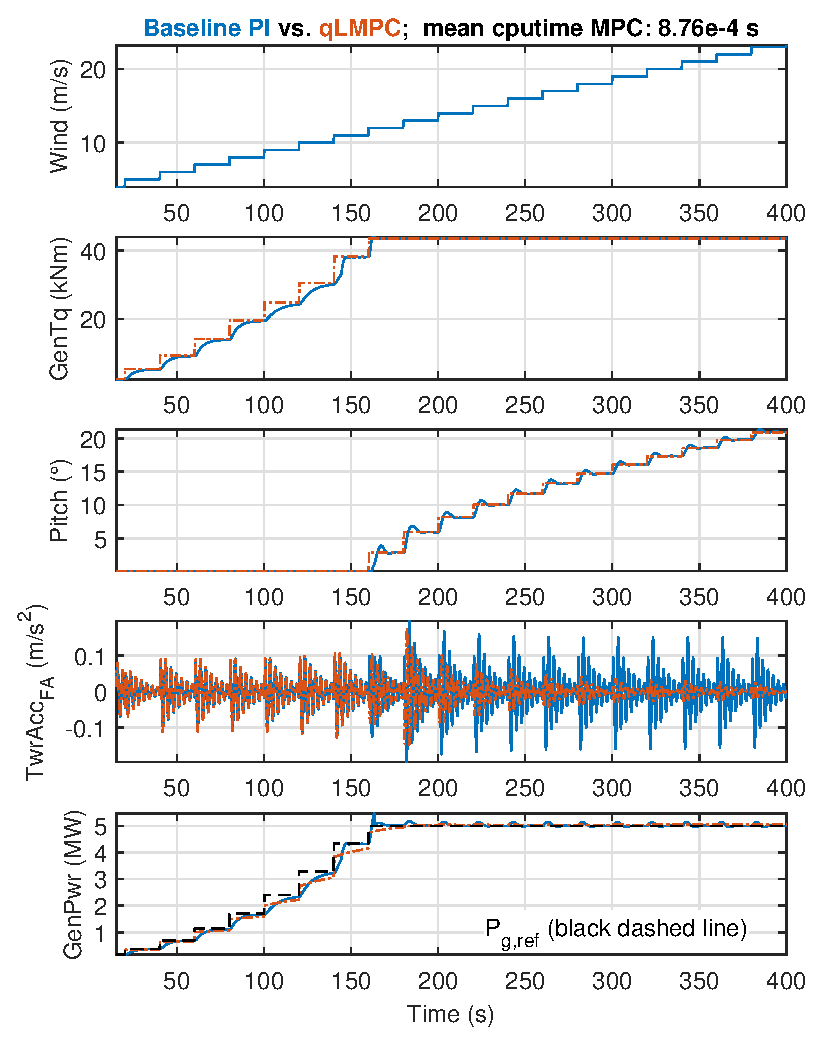
\includegraphics[width=0.485\textwidth]{figures/Figures_ADi/cmpCtrlTimeDomain_All_RefSimulinkClosedLoop_beta.eps}}\hfill 
    \subfloat[Turbulent wind, IEC class B, 18~m/s mean speed]{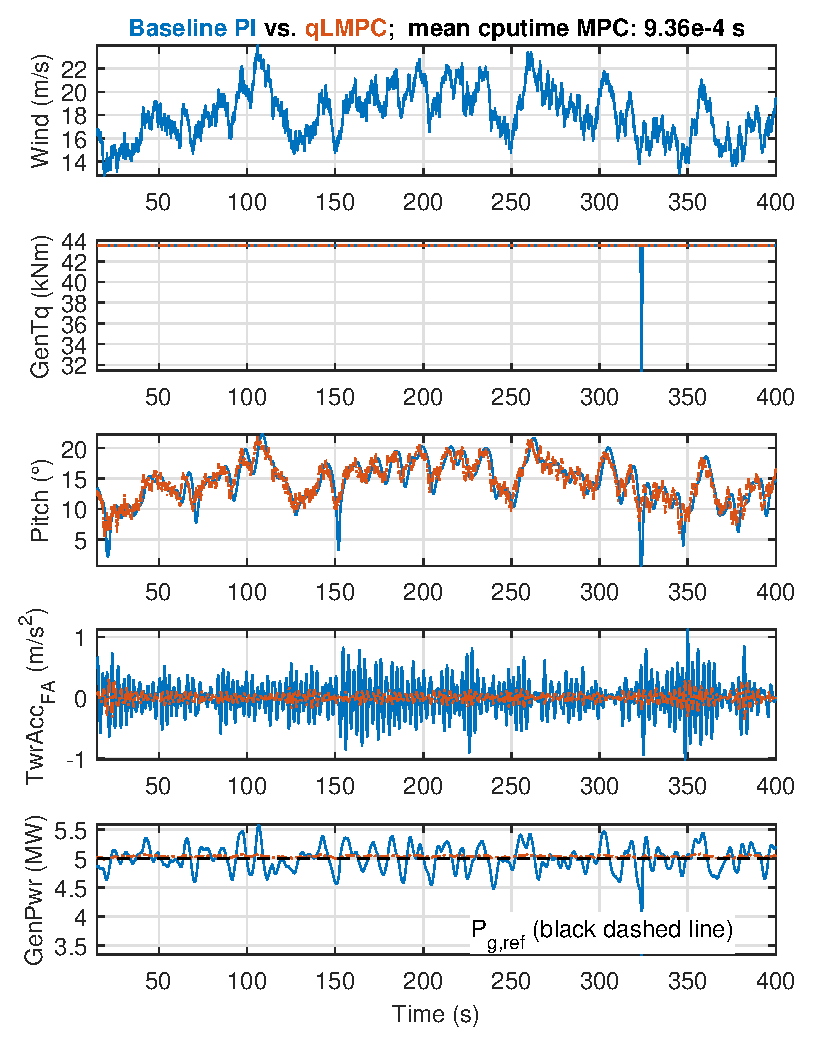
\includegraphics[width=0.485\textwidth]{figures/Figures_ADi/cmpCtrlTimeDomain_All_RefSimulinkClosedLoopNTW18_beta.eps}}\hfill
    %\subfloat[blc blc]{\includegraphics[width=0.31\textwidth]{figures/twoTurbinesGreedyOpt_2d.eps}}
    \caption[Controller comparison: qLPV model with baseline 
    PI controller vs. qLMPC for stepped wind sweep and turbulent wind.]{Controller comparison: qLPV model with baseline 
        PI controller vs. qLMPC for stepped wind sweep and turbulent wind (18\,m/s mean, IEC turbulence 
        class B (14\%)).  PI control (blue line), qLMPC (red line) and power reference (black dashed line). Displayed signals: wind speed, control inputs, tower fore-aft
        accelerations, and power output.}
    \label{fig:CtrlCmpMdlSweep}
\end{figure}

 The QP is solved using a linear complementary problem formulation with Lemke's algorithm \cite{cisneros2020velocity}, which enables fast convergence, as real-time capability is a critical requirement for online optimization-based control. Of the 50001 controller cycles at a sampling time of 8\,ms needed for the 400\,s simulation time, only one cycle exceeded the sampling time and only 13 exceeded 2\,ms. The mean CPU time remained considerably below 2\,ms, as shown in the subplot titles of Figure~\ref{fig:CtrlCmpMdlSweep}. These measurements were obtained in MATLAB R2021b on an Intel Core i7-11850H (2.5\,GHz, 8 cores) running Windows 10. Note that for deployment on a physical turbine, a fallback strategy would be required to handle the rare cases where the solver exceeds the sampling time. This was not implemented in this proof-of-concept, but several options exist, such as blending the last available qLMPC solution with the output of the PI feedback controller.

However, the improvements regarding the reduction of tower acceleration and power variance come at the price of higher actuation rate.
Table \ref{tab:ControllerComparisonMerged} summarizes this by displaying the afore mentioned changes in tower fore-aft acceleration and power tracking error as standard deviation for physical interpretability for both the baseline PI controller and the qLMPC algorithm.  
\begin{table}[t]
    \centering
    \caption[Standard deviation comparison: Baseline PI vs.\ qLMPC for stepped wind sweep and
    turbulent wind.]%
    {Standard deviation comparison: Baseline PI vs.\ qLMPC for stepped wind sweep and
        turbulent wind (18\,m/s mean, IEC class B).
        The standard deviations obtained with the PI controller are divided by those obtained with the qLMPC; quotients above~1 indicate improvement.} %In the turbulent wind case, both controllers operate at rated   generator torque throughout, resulting in zero torque rate standard  deviation for both
    \label{tab:ControllerComparisonMerged}
    \begin{tabular}{l rr}
        \toprule
        {Standard Deviation of} & {Stepped wind sweep} & {Turbulent wind} \\
        {Signal (unit)} & \multicolumn{2}{c}{std PI / std qLMPC =  ratio} \\
        \midrule
        Tower fore-aft acceleration (m/s$^2$) & $0.06 / 0.03 = 1.77$ & $0.17 / 0.07 = 2.31$ \\
        Power tracking error (kW) & $169.01 / 146.26 = 1.16$ & $56.68 / 14.68 = 3.86$ \\
        Generator torque rate (kNm/s) & $0.63 / 2.36 = 0.27$ & $0 / 0 = {-}$ \\
        Blade pitch rate (\textdegree/s) & $0.22 / 0.81 = 0.27$ & $0.51 / 3.60 = 0.14$ \\
        \bottomrule
    \end{tabular}
\end{table}
%
%\\begin{tablenotes}
 %   \small
%    \item In the turbulent wind case, both controllers operate at rated 
%    generator torque throughout, resulting in zero torque rate standard 
%    deviation for both.
%\end{tablenotes}
%
Ratios above~1 indicate improvement, confirming the qLMPC reduces both tower loading and power tracking error.  But the standard deviation in rates in blade pitch increase, for the turbulent wind test case even considerably so. There is also a decrease in generator torque observed for the stepped wind test case. In the turbulent wind case, both controllers operate at rated generator torque throughout, resulting in zero torque rate standard  deviation for both. As more improvement in power variance was observed for the above rated turbulent wind, the following discussion focuses on this case.

For the results of this proof-of-concept, visualized in Figure~\ref{fig:CtrlCmpMdlSweep}, no penalty is placed on pitch actuator movement, and the pitch rate limit is set to 13\textdegree/s, which is a relatively high value. Figure~\ref{fig:CtrlCmpRates} shows the results of six test runs with different pitch rate limits: three with the baseline PI controller and three with the qLMPC algorithm. The effect of different pitch rates on the PI controller is depicted in Figure~\ref{fig:CtrlCmpRates}(a), and on the qLMPC design in Figure~\ref{fig:CtrlCmpRates}(b). The selected pitch rate limits of 4\textdegree/s, 8\textdegree/s, and 13\textdegree/s represent a range from conservative to highly responsive actuator capabilities. They were chosen to explore both realistic hardware limitations and the potential performance gains of faster actuation.

The signals shown for both investigated control algorithms are the wind speed, collective blade pitch angle, rotor speed, fore-aft tower acceleration, and generator power. It should be noted that generator torque does not change at all in this above-rated test case and is hence not shown. Under baseline PI control, increasing the pitch rate shows very little effect, as the rotor acts as a filter in this pure feedback design. In contrast, the qLMPC controller shows a considerable difference when only 4\textdegree/s pitch rate is allowed compared to the two higher rates. Allowing a pitch rate of approximately 8\textdegree/s or faster improves rotor speed regulation and reduces both tower movement and power variability by more than a factor of 3. However, it also leads to higher pitch activity.  The qLMPC reduces the variance of rotor speed, tower fore-aft movement, and power output for all rate limits, even at a  4\textdegree/s rate limit. However, the qLMPC benefits from higher pitch rates, as faster pitch response enables better disturbance rejection. The trade-off between actuator activity on the one hand and load reduction and smoother power output on the other is ultimately a design decision, which may also vary over the turbine's lifetime as the pitch bearings age.

\begin{figure}[h]
    \subfloat[Baseline PI controller]{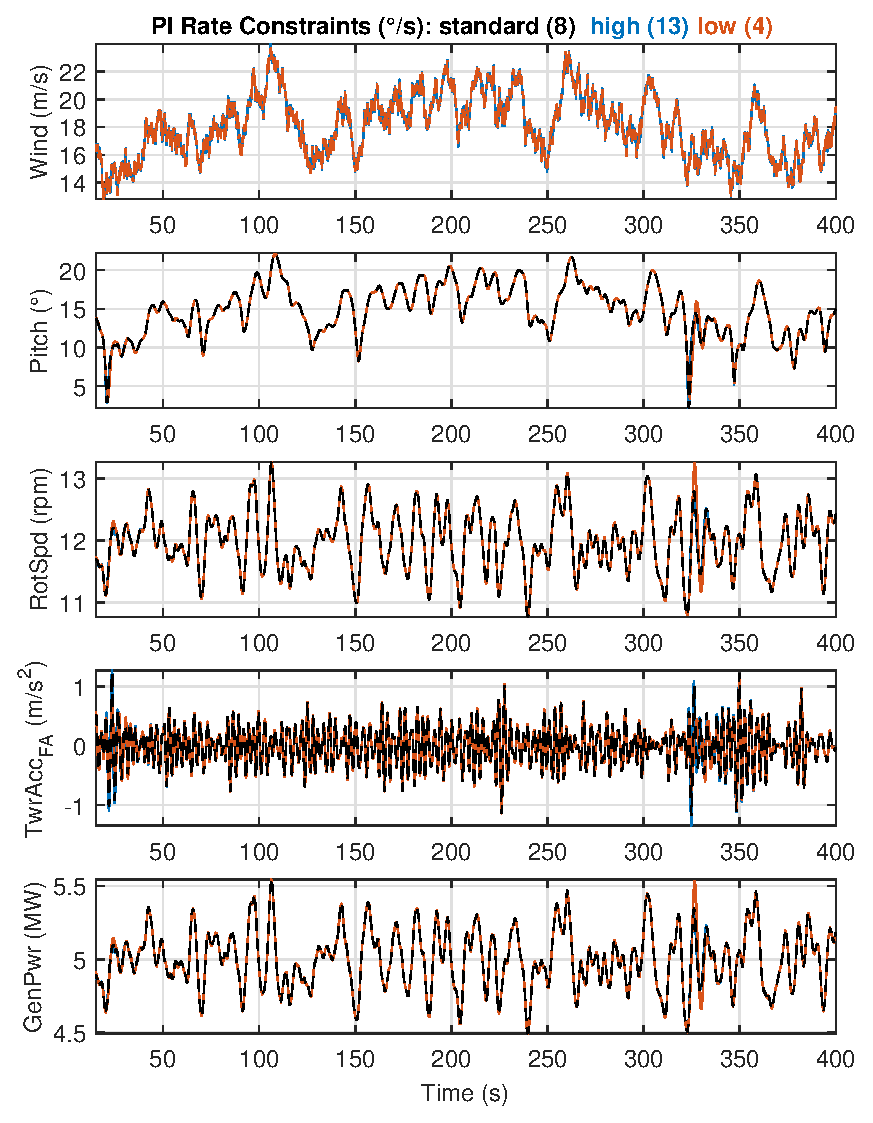
\includegraphics[width=0.485\textwidth]{figures/figDirConstr1/cmpTimeDomain_All5PINewLim.eps}}\hfill 
    \subfloat[qLMPC algorithm]{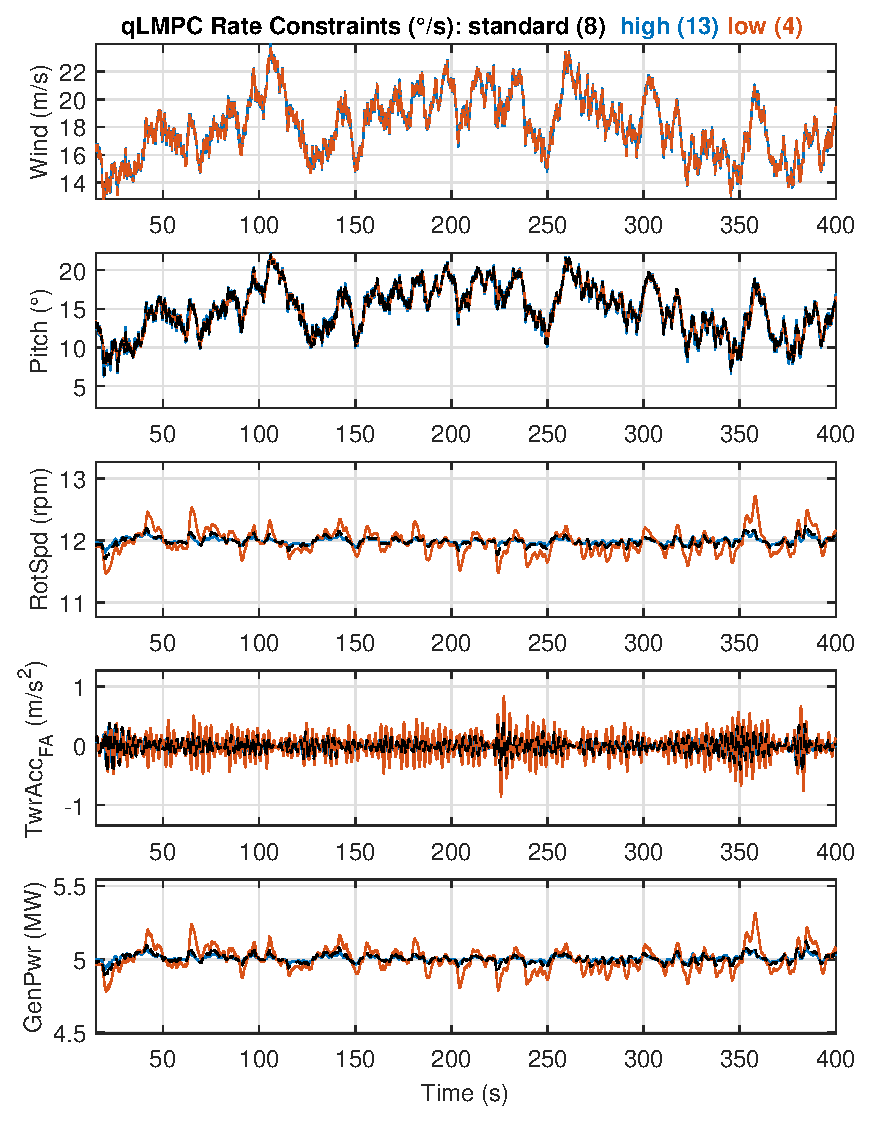
\includegraphics[width=0.485\textwidth]{figures/figDirConstr1/cmpTimeDomain_All5MPCNewLim.eps}}\hfill
     \caption[Controller comparison: Baseline PI and qLMPC with different pitch rate limits.]{Controller comparison: Baseline PI and qLMPC with different pitch rate limits for turbulent wind (18\,m/s mean, IEC turbulence  class B (14\%)). Rate limits: Standard 8\textdegree/s~(black line), high 13\textdegree/s~(blue line), and low 4\textdegree/s~(red line)). Displayed signals: wind speed, pitch, states, and power.}
    \label{fig:CtrlCmpRates}
\end{figure}

The standard deviations of the pitch derivative, the rotor speed, the tower fore-aft acceleration and the generated power for Figure~\ref{fig:CtrlCmpRates} are summarized in Table~\ref{tab:stddev_unified}.

\begin{table}[htbp]
    \centering
    \caption[Standard deviation comparison: Baseline PI vs.\ qLMPC for turbulent wind with different pitch rate limits.]%
    {Standard deviation comparison: Baseline PI vs.\ qLMPC
        for turbulent wind with pitch rate limits. The PI controller is largely insensitive to the rate limit
        whereas the qLMPC uses higher rates for less rotor speed, tower movement and
        power variation. Values in brackets show the ratio to the standard
        (8\textdegree/s) baseline PI value.}
    \label{tab:stddev_unified}
    \begin{tabular}{ll rrr}
        \toprule
        & & \multicolumn{3}{c}{Rate limit (\textdegree/s) (ratio to PI at 8\textdegree/s)} \\
        \cmidrule(lr){3-5}
        Controller & Signal & low: 4\textdegree/s & standard: 8\textdegree/s & high: 13\textdegree/s \\
        \midrule
        \multirow{4}{*}{PI}
        & Tower fore-aft acc.\ (m/s$^2$) & 0.32 (1.03) & 0.33 (1.00) & 0.34 (0.97) \\
        & Generated power (kW) & 200.26 (0.99) & 197.62 (1.00) & 197.32 (1.00) \\
        & Rotor speed (rpm) & 4.57 (0.99) & 4.51 (1.00) & 4.50 (1.00) \\
        & Blade pitch rate (\textdegree/s) & 1.21 (1.06) & 1.28 (1.00) & 1.34 (0.96) \\
        \midrule
        \multirow{4}{*}{qLMPC}
        & Tower fore-aft acc.\ (m/s$^2$) & 0.21 (1.57) & 0.11 (3.00) & 0.08 (4.12) \\
        & Generated power (kW) & 78.37 (2.52) & 30.72 (6.43) & 19.63 (10.07) \\
        & Rotor speed (rpm) & 1.79 (2.52) & 0.70 (6.44) & 0.45 (10.02) \\
        & Blade pitch rate (\textdegree/s) & 1.84 (0.70) & 3.11 (0.41) & 3.88 (0.33) \\
        \bottomrule
    \end{tabular}
\end{table}

The application of the proposed velocity-based qLMPC concept significantly reduces tower movements and minimizes power output fluctuations. As noted at the start of this section, DEL reduction is not directly a qLMPC objective. However, it will be shown in Section~\ref{subsection: IPCResults} and~\ref{subsec:ComparisonWindTurbineControlDesigns} that the reduced tower movement also results in considerably reduced Damage Equivalent Loads (DELs) and the corresponding values are included in comparisons with other control schemes in the Figures~\ref{fig:EvalCrit1} and~\ref{fig:CtrlCompAll}.

The performance improvement comes at the cost of requiring accurate wind information, either obtained through expensive sensors such as lidars or through wind estimations. A purely feedback-based improvement over standard collective pitch control is individual pitch control, which uses blade root moments and rotor azimuth position as additional feedback signals and is already widely deployed in commercial turbines. This approach is widely investigated in both theoretical studies and field tests and has proven to be an effective strategy, either as an alternative or in addition to MPC, to further reduce mechanical loads. While its primary focus is on reducing blade loads, a reduction in tower loads is also possible, as will be discussed in the next section.

